\subsection{Software design}
\label{sec:programmingModel}

% \ad{Attestation and platform awareness part is revised. Continue with the motivation}

In this section, we introduce \name{}'s software design which is one possible way for the application, driver, and firmware developers to adapt their software to be compatible with \name without making a significant changes.  

% \begin{figure}[t]
% \centering
% 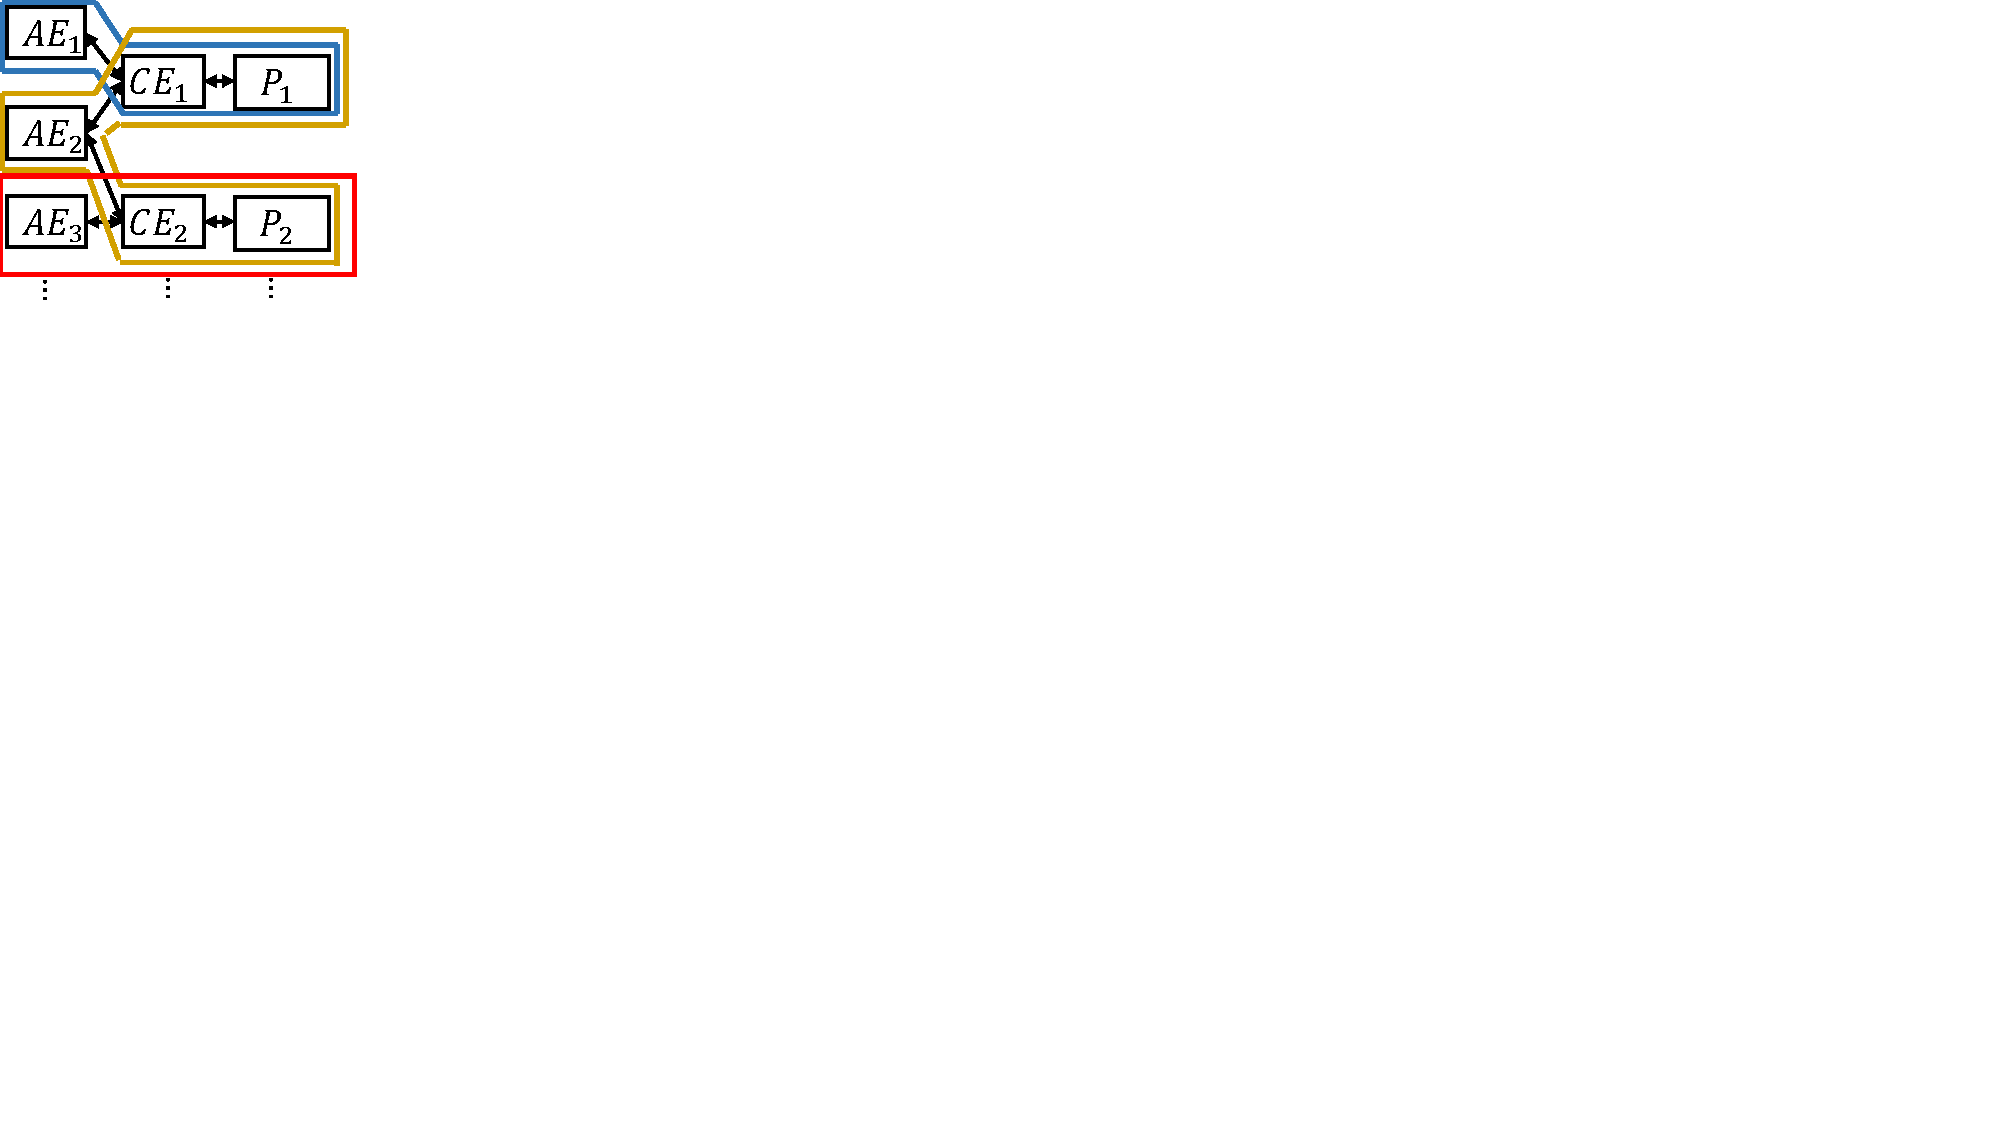
\includegraphics[trim={0 14cm 27cm 0}, clip, width=0.5\linewidth]{programmingModelComponents.pdf}
% %\caption{\textbf{\Nameenclave{}s in the \name{}'s software design.} The application enclaves (AE) contain the application logic and communicate with \sphw through a controller enclave (CE) that contain the driver logic for the specific \sphw. In our software design, we assume that there is only one \ce per \sphw. Multiple \app can connect to one \ce{}, and one \app can connect to multiple \ce. Three separate \nameenclave{}s are indicates by the blue, yellow and red outlines.}
% \vspace{-1em}
% \caption{Three example \nameenclave{}s in \name{}'s software design with \app{}s (AE), \ce{}s (CE), and \sphw{} devices (P). Note that the yellow \nameenclave{} is spanning two external devices. It is the responsibility of the \ce{}s to isolate the data from the different \app{}s.}
% \label{fig:programmingModelComponents}
% \end{figure}

\subsubsection{Software components}
\label{sec:programmingModel:systemComponents}

\name's software design consists of three entities: \app{}s, \ce{}s, and \sphw firmware as shown in Figure~\ref{fig:sharedMemory}. \app{}s and \ce{}s are processor-local enclaves. \sphw are the components that are connected to the platform over buses. Contrary to a monolithic design where the application and driver is in one big enclave, our modular approach aims to provide high flexibility and increase code reuse.

\setcounter{para}{0}

\mypara{Application enclaves} \App{}s are similar to the traditional enclaves in Intel SGX or Keystone. In such TEEs, the enclaves cannot access \sphw without using the OS as a mediator, as the OS handles all drivers. In \name, \app{}s also cannot communicate with a \sphw directly. The \app{}s use shared memory to communicate with a \ce that is a \sphw-specific enclave containing the driver logic. The rationale of separating the driver from the application logic is two-fold, i) to avoid requiring the developers to ship driver code with their application, and ii) one \ce per \sphw allows multiple \app{}s to communicate with that specific \sphw in parallel. %Note the processor may employ memory encryption to encrypt all shared memory regions to protect against a local physical attacker. However, the developer could also add an additional encryption layer on top in order to make the data accessible only between the application enclave and the \sphw (where the \ce works as the untrusted transport layer between the \app and the \sphw). 


\mypara{Controller enclave} The \ce contains the driver that facilitate communication with a \sphw. Note that \app{}s, standard non-enclave applications, and the OS cannot access the \sphw directly. The only way to communicate with a \sphw is through a device-specific \ce. Such a design choice isolates the \sphw drivers: one compromised driver does not affect other \sphw. The \ce maintains an isolated communication channel over shared memory (e.g., in RISC-V, the PMP entry corresponding to a shared memory ensures that only participating enclaves have access to that shared memory) to \app{}s and the \sphw. To simplify the configuration, we assume that only one active \ce per \sphw exists at a time. However, any \ce can be replaced at the user's request. %Note that \ce is the only way to access a specific peripheral. All the other non-enclave applications running on the OS need to connect the \ce (in contrast to the standard OS device driver) to access a peripheral.  

\subsubsection{Isolation of multi-\app session}\label{sec:programmingModel:systemComponents:multiApp} In \name, multiple \app{}s could connect to a single \ce to have simultaneous access to a \sphw. In such a scenario, the \ce keeps separate states corresponding to each of the \app{}s. Note that this is primarily a functional and then a security requirement as operations in one \app could affect the state of computation of another \app in case there is no isolation. For some \sphw, the \ce may need to reset the state of the \sphw when it switches to a session with a different \app (temporal separation). However, for \sphw such as GPU that support multiple isolated workloads in parallel, the state does not have to be reset.


\subsubsection{Platform-wide attestation in the software design}

The platform-wide attestation enables a remote verifier to verify the state of the all \nameenclave components. The attestation proceeds as the following:

\setcounter{para}{0}
\mypara{Remote attestation of the \app} This is the first step of the  platform-wide attestation to ensure that the platform is running the intended version of the \app. The \app attestation report includes the list of identifiers of the \ce{}s that have shared memory channels with that \app.
    
\mypara{Remote attestation of the connected \ce{}s} The user then executes a series of individual remote attestation for the \ce{}s. The \ce{}s send the attestation report of themselves along with the certificate that is received from the connected \sphw. These reports are signed by the same platform key as of the \app attestation report. This proves that the \app and the connected \ce{}s are running on the same physical platform. Additionally, the \ce also states that the initiating \app has a shared memory channel with it.
\setcounter{para}{0}

%===========================================================================================================
% \paragraph{Remote attestation of the \app} The platform-wide attestation process starts with the verifier who wants to attest the deployed \app. The purpose of the remote attestation of the \app is to ensure that the platform is running the intended version of the \app. The \app attestation report includes the list of identifiers of the \ce{}s that have shared memory channels with that \app. This report is signed by the platform's private key. 

% \paragraph{Remote attestation of the connected \ce{}s} As mentioned above, the user receives a list of identifiers of \ce{}s that have shared memory channel with the \app. The user then executes a series of individual remote attestation for the \ce{}s. The \ce{}s send the attestation report of themselves along with the certificate that is received from the connected peripherals. These reports are signed by the same platform key as of the \app attestation report. This proves that the \app and the connected \ce{}s are running on the same physical platform. Additionally, the \ce also states that the initiating \app has a shared memory channel with it. At the end of this process, the verifier who initiated the remote attestation of the \app receives the signed attestation report of the said \app, all the \ce{}s that are connected with the \app and all the peripherals that are governed by the \ce{}s.

% \paragraph{Local attestation between \ce and peripheral} The local attestation process between a peripheral and a \ce takes place when a new peripheral is attached to the platform. This step is independent of the above mentioned two steps that only starts when the verifier wants to attest a specific \app. When a new peripheral is attached to the platform, \ce gets the list of attached peripherals from the SM (through the device tree). The peripherals come with a certificate that states the firmware version certified by the manufacturer along with the signing key from the manufacturer. The \ce issues a random challenge to the peripheral. It verifies if the peripheral actually owns the private key corresponding to the certificate. The peripheral signs the challenge and sends it back to the \ce for verification.
% After the local attestation between the \ce and the peripheral, the \ce knows that is it connected with a legitimate peripheral with a certified firmware.



% \paragraph{Peripherals} 
% \label{sec:programmingModel:systemComponents:peripheral}

% We consider on-chip peripherals as well as external peripherals that are attached to the platform. However, we require them to store some key material from the manufacturer securely for attestation. Similar to \app{}s, peripherals also share memory regions with the \ce that is used as a communication channel. The firmware that runs on peripherals is also part of the platform-wide enclaves. For simple peripherals such as IO devices (keyboard, mouse, etc.), GPS, and temperature sensors, the modification in the firmware is minimal. Essentially, this only includes adding a certificate from the manufacturer that proves that the peripheral is running the correct version of the firmware. %However, for complex peripherals such as GPUs, the developers may require to change the firmware as the GPU needs to isolate the data from multiple \app{}s that execute operations on the GPU simultaneously.



% \subsection{Platform-wide Attestation}
% \label{sec:programmingModel:attestation}

% In Section~\ref{sec:approach:attestation}, we provide the hardware construct for \name{}'s platform-wide attestation. In this section, we describe how it related to the programming model components. The platform-wide attestation that enables a remote verifier to verify the state of the \nameenclave components - \app{}s, \ce{}s, and peripherals. Precisely, the state includes the state of the components of the programming model components and their communication channel (over shared memory in our case). Note that there could be more than one verifier (an example is depicted in Figure~\ref{fig:new_system} with two remote verifiers and two \nameenclave{}s) corresponding to several \nameenclave{}s on the same platform. For each remote verifier, the TCB is constrained to only the specific \nameenclave that she is verifying. Hence a remote verifier does not need to trust any \app, \ce or peripheral that she is not using/attesting. Note that platform-wide attestation is built on top of the attestation scheme of the underlying TEE, e.g., the attestation in RISC-V Keystone or Intel SGX. %Enabling  platform-wide attestation requires some modifications of the existing remote attestation procedure of traditional TEEs. 



